\documentclass{article}

\usepackage{../preamble}
\standalonetrue

\pagestyle{fancy}
\fancyhf{}
\rhead{Section \thesection}
\lhead{PHYS 304 Lecture 5}
\rfoot{Page \thepage}


\title{PHYS 304 Lecture 5}
\author{Ashtan Mistal}
\date{!!!}

\begin{document}

\ifstandalone
\maketitle
\fi

\graphicspath{{./Lecture05/}}

\section{Key points from last day}

By using separation of variables, the partial differential, spatio-temporal Schrödinger equation reduces to two separate differential equations for the time- and space-independent Schrödinger equations.


The space-independent equations is straight forward to solve, and doesn't really depend on initial conditions (the normalization factor is subsumed in the time-independent solution).  The solution is$e^{- \frac{i E}{\hbar} t}$ , where $E$ is a number that also enters the time-independent Schrödinger equation (and thus intimately connects them).

The time-independent equation is in general more difficult to solve, and it does depend on boundary conditions, that typically restrict the shape of the spatial wavefunction and the allowed values of $E$ to a set  $\{ E_n\}$ while its amplitude is obtained from the normalization requirement.  Each solution for an allowed value of $E_n$, $\psi_n(x)$, has a corresponding temporal dependence $\phi_n(t) = e^{- \frac{i E}{\hbar} t}$, so the complete stationary solution is $\Psi_n(x,t) = \Psi_n(x) e^{- \frac{i E}{\hbar} t}$. 

If a particle is in any one of the stationary state solutions of Schrödinger equation labelled by $n$ (but not in a superposition of such states), the expectation value of any physical observable is independent of time, and the expectation value of the energy is $E_n$, with zero variance (the energy of a stationary state is precisely defined).


\section{Today: Solving the Schrodinger Equation}

Crucially, the entire set of all solutions of the time-independent Schrödinger equation, with their corresponding values of $E_n$ , form a complete orthonormal set of functions that can be used to expand an arbitrary spatially varying function defined in the region where the particles exist, satisfying the same boundary conditions.   

The algorithm (flowchart) for solving the full Schrödinger equation using separation of variables is [from text]:

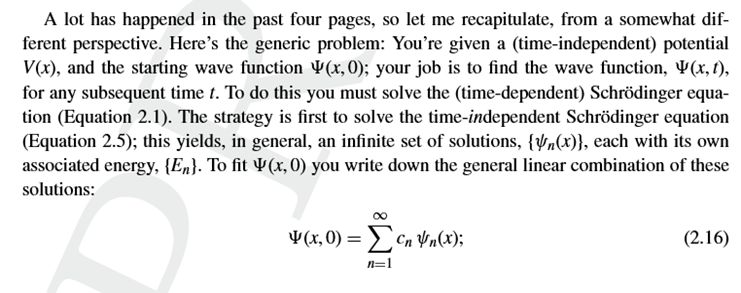
\includegraphics[width = 0.8 \textwidth]{Lecture05/1.png}

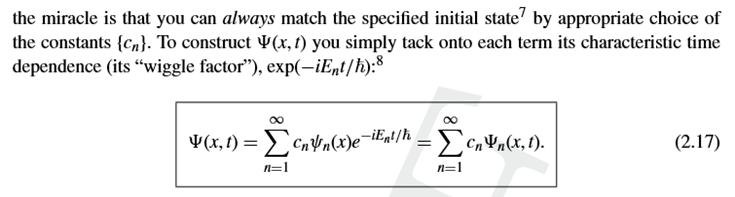
\includegraphics[width = 0.8 \textwidth]{Lecture05/2.png}

This holds similarity to classical mechanics where we have to be given the potential, and the position and velocity of the particle at t=0.

The first step is to solve the time-independent SE.

Next, expand initial wavefunction in the eigen states of the TISE (emphasizing similarity but generalization of Fourier series expansion that we went through in tutorial yesterday)

Getting the full time dependence is of trivial nature. Note that the general wavefunction is NOT harmonic. 

\section*{Crucial concept}

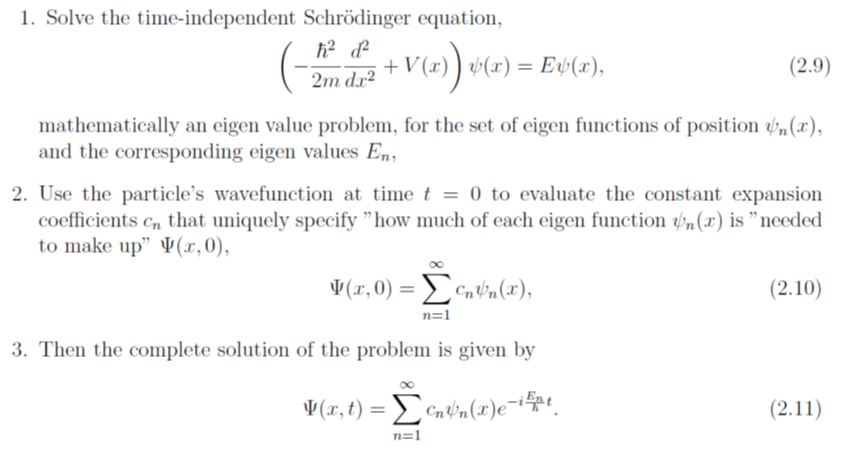
\includegraphics[width = 0.8 \textwidth]{Lecture05/3.png}

This makes the time dependence part of a solution "trivial". 

\section{Infinite square well potential}

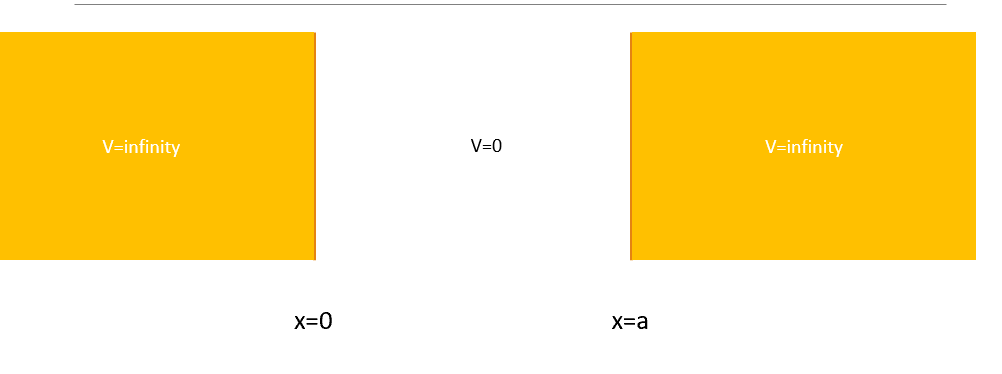
\includegraphics[width = 0.8 \textwidth]{Lecture05/4.png}

\subsection{Activity 1}

\begin{enumerate}
    \item Sketch the potential, $V(x)$, for $- \infty < x < \infty$. 
    \item Solve the time-independent SE separately in the three regions: $x < 0, 0 < x < a, x > a$, leaving the solutions in their most general form, with unknown coefficients, at this stage. 
\end{enumerate}

Regarding infinite square well solutions of the TISE, when $V(x)$ is infinite, then classically and quantum mechanically there is no probability that the particle can be located in that region. The implication is that the wavefunction must be zero in this problem, except for $0 < x < a$, where $V(x) = 0$. So, for $0 < x < a$, the time independent SE is:

$$\left( \frac{- \hbar^2}{2m} \frac{d^2}{dx^2} + 0 \right) \psi(x) = E \psi(x)$$

\subsection{Activity 2}

Use the fact that the wavefunction has to be continuous in $- \infty < x < \infty$, to find the allowed values of $E_n$. 

The continuity of $\psi(x) \Rightarrow \psi(x = 0) = \psi(x= a) = 0$. 

Why is $E_n$ restricted to positive values, physically? Why did we not have to use the $x = a$ boundary condition?

\begin{itemize}
    \item $E=0$ solution is boring, because the wavefunction is zero everywhere. 
    \item $E < 0$ can't satisfy the boundary conditions, since we have real exponential functions
\end{itemize}

\subsection*{What do we know about the solutions of the TISE for an infinite square well of width $a$?}

$\psi_n(x) \propto \sin \left( \frac{n \pi x}{a} \right)$ singe $A = -B$, and the sassociated values of $E_n$ are $E_n = \frac{\hbar^2}{2m} \left( \frac{n \pi}{a} \right)^2, n = 1,2,...$. There are no other allowed values of $E$!

Next?

\subsection{Orthogonal and Orthonormal Functions}

Recall the key step in the recipe is to find the $\{c_n\}$ in: $\Psi(x,0) = \sum_{n=1}^\infty c_n \psi_n(x)$.

What does it mean for two functions to be “orthogonal”? Write a defining equation.  What is the difference between orthogonal and orthonormal? 

$$\int \psi_m(x)^* \psi_n(x) dx = 0, (m \neq n)$$

$$\int \psi_m(x)^* \psi_n(x) dx = \delta_{mn}$$

What does it mean for a set of functions to be "complete"? Use equations and provide an explanation. 

$$f(x) = \sum_{n=1}^\infty c_n \psi_n(x)$$

One must emphasize the similarity to a 2D vector decomposition, and to Fourier series, but recognize this is more general now, since the expansion functions are solutions of TISE, not necessarily a set of harmonic sinusoids (although in this case they are a set of harmonic sinusoids!). 

Note that this must be a unique set of $c_n$. 


\hfill

Show that the $\psi_n(x) = \sqrt{\frac{2}{a}} \sin \left( \frac{n \pi x}{a} \right)$ are orthonormal. 

For this, we need to show the following:

$$\frac{2}{a} \int_0^a \sin \left( \frac{n \pi x}{a} \right) \sin \left( \frac{m \pi x}{a} \right) dx = \delta_{mn}$$

Note the trigonometric identities useful in solving this and others:

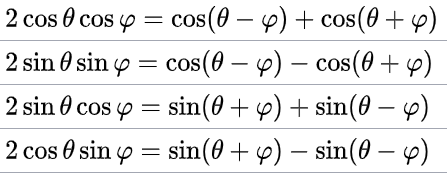
\includegraphics[width = 0.4 \textwidth]{Lecture05/5.png}



\end{document}